% This file was generated with po4a. Translate the source file.
%
\chapter{Benutzerhandbuch}


\section{Das Web-Interface}
Sie können sich mit einem beliebigen Webbrowser mit Ihrer PDR-Instanz
verbinden. Navigieren Sie einfach zu Ihrem Server und geben Sie Ihren
Benutzernamen und Ihr Passwort ein.

\subsection{Login}
\begin{figure}[h]
	\centering
	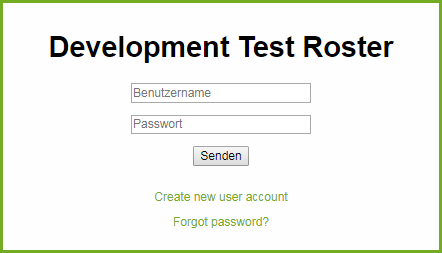
\includegraphics[width=.3\linewidth]{{images/en_GB/login.php}.png}
	\caption{Login Seite}
\end{figure}
Die Anmeldeseite zeigt den Namen der Anwendung an. Sie werden aufgefordert,
Ihren Benutzernamen und Ihr Passwort einzugeben. Wenn Sie noch keinen
Account haben, können Sie \menu{Create a new account} erstellen. Wenn Sie
ein Konto haben, aber Ihr Passwort vergessen haben oder es ändern möchten,
können Sie auf \menu{Passwort vergessen?} Klicken.


\subsection{Neuen Benutzer-Account erstellen}
\begin{figure}[ph]
	\centering
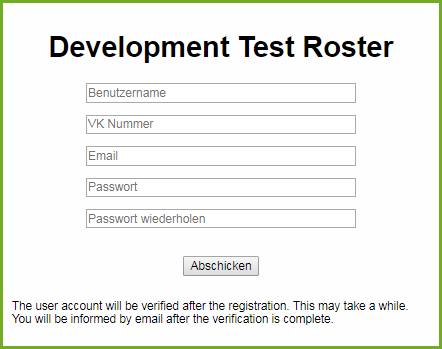
\includegraphics[width=0.4\linewidth]{{images/en_GB/register.php}.png}
	\caption{Registrierungsseite}
\end{figure}
Wählen Sie einen Benutzernamen, geben Sie Ihre Mitarbeiter-ID und Ihre
E-Mail-Adresse ein. Wählen Sie ein sicheres Passwort.

Das Konto ist inaktiv, bis ein Administrator es aktiviert. Der
Hauptadministrator wird per E-Mail über die Registrierung informiert.

Neue Benutzer können nur für vorhandene Mitarbeiter erstellt werden. Neue
Mitarbeiter werden von einem Administrator erstellt. 

\subsection{Passwort vergessen}
\begin{figure}[h]
    \centering
    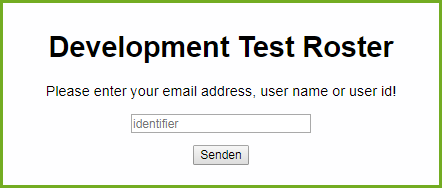
\includegraphics[width=.3\linewidth]{{images/en_GB/lost_password.php}.png}
    \caption{Passwort vergessen Seite}
\end{figure}
Auf der Seite "Passwort vergessen" wird der Name der Anwendung
angezeigt. Sie werden aufgefordert, entweder Ihren Benutzernamen, Ihre ID
oder Ihre E-Mail-Adresse einzugeben. Nachdem Sie das Formular abgeschickt
haben, wird eine E-Mail an Ihre gespeicherte E-Mail-Adresse gesendet. In
dieser E-Mail finden Sie einen Link, der Sie zur Seite zum Ändern des
Passworts führt.
\subsubsection{Wiederherstellung des Passwortes}
\begin{figure}[ph]
    \centering
    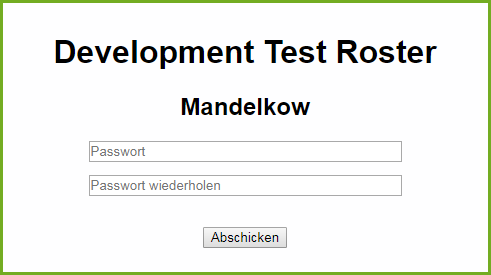
\includegraphics[width=0.3\linewidth]{{images/en_GB/reset-lost-password.php}.png}
    \caption{Wiederherstellungs-Seite für Passwörter}
\end{figure}
Auf der Seite zur Wiederherstellung des verlorenen Passworts werden der Name
der Anwendung und Ihr Benutzername angezeigt. Sie werden aufgefordert, ein
neues Passwort zweimal einzugeben.


\subsection{Navigation}
\begin{figure}[ph]
	\centering
	
\includegraphics[width=0.8\linewidth]{{images/en_GB/navigation}.png}
	\caption{Navigationsleiste}
	\label{img_navigation_bar}
\end{figure}
Standardmäßig öffnet die PDR-Weboberfläche ein Menü mit 5 Kacheln. Sie
können navigieren zu:
\begin{itemize}
\item Dienstplan Wochenansicht 
\includegraphics[height=2em]{../img/md_view_week-24px}
\item Dienstplan Tagesansicht 
\includegraphics[height=2em]{../img/day}
\item Dienstplan Mitarbeiteransicht 
\includegraphics[height=2em]{../img/employee_2}
\item Überstunden  
\includegraphics[height=2em]{../img/watch_overtime}
\item Abwesenheit 
\includegraphics[height=2em]{../img/absence}
\end{itemize}

\subsubsection{Die Navigationsleiste}
Im oberen Bereich befindet sich eine Navigationsleiste mit Hyperlinks zu
fast allen PDR-Seiten. Bewegen Sie die Maus über einen Eintrag, um die
Untermenüs zu öffnen (\autoref{img_navigation_bar}).
\begin{multicols}{3}
\begin{description}
    \item \menu{Wochenansicht > .. }
    \begin{description}
        \item \menu{.. > Wochen-Tabelle}
        \item \menu{.. > Wochen-Bilder}
    \end{description}
    \item \menu{Tagesansicht > .. }
    \begin{description}
    \item \menu{.. > Tagesansicht Eingabe}
    \item \menu{.. > Tagesansicht Ausgabe}
    \item \menu{.. > Grundplan Tagesansicht}
    \end{description}
    \columnbreak
    \item \menu{Mitarbeiter > .. }
    \begin{description}
    \item \menu{.. > Mitarbeiteransicht}
    \item \menu{.. > Grundplan Mitarbeiter}
    \end{description}
    \item \menu{Überstunden > ..}
    \begin{description}
    \item \menu{.. > Überstunden Eingabe}
    \item \menu{.. > Überstunden Ausgabe}
    \item \menu{.. > Überstunden Übersicht}
    \end{description}
    \item \menu{Abwesenheit > ..}
    \begin{description}
    \item \menu{.. > Abwesenheit Eingabe}
    \item \menu{.. > Abwesenheit Jahresplan}
    \item \menu{.. > Abwesenheit Monatsplan}
    \end{description}
    \columnbreak
    \item \menu{Administration > ..}
    \begin{description}
    \item \menu{.. > Anwesenheitsliste}
    \item \menu{.. > Samstagsliste}
    \item \menu{.. > Stundenzettel geringfügig Beschäftigte}
    \item \menu{.. > PEP-Upload}
    \item \menu{.. > Mitarbeiterverwaltung}
    \item \menu{.. > Mandantenverwaltung}
    \item \menu{.. > Benutzerverwaltung}
    \item \menu{.. > Konfiguration}
    \item \menu{.. > phpMyAdmin}
    \end{description}
\end{description}
\end{multicols}
\subsection{Dienstplan Wochenansicht}
\begin{figure}[h]
	\centering
	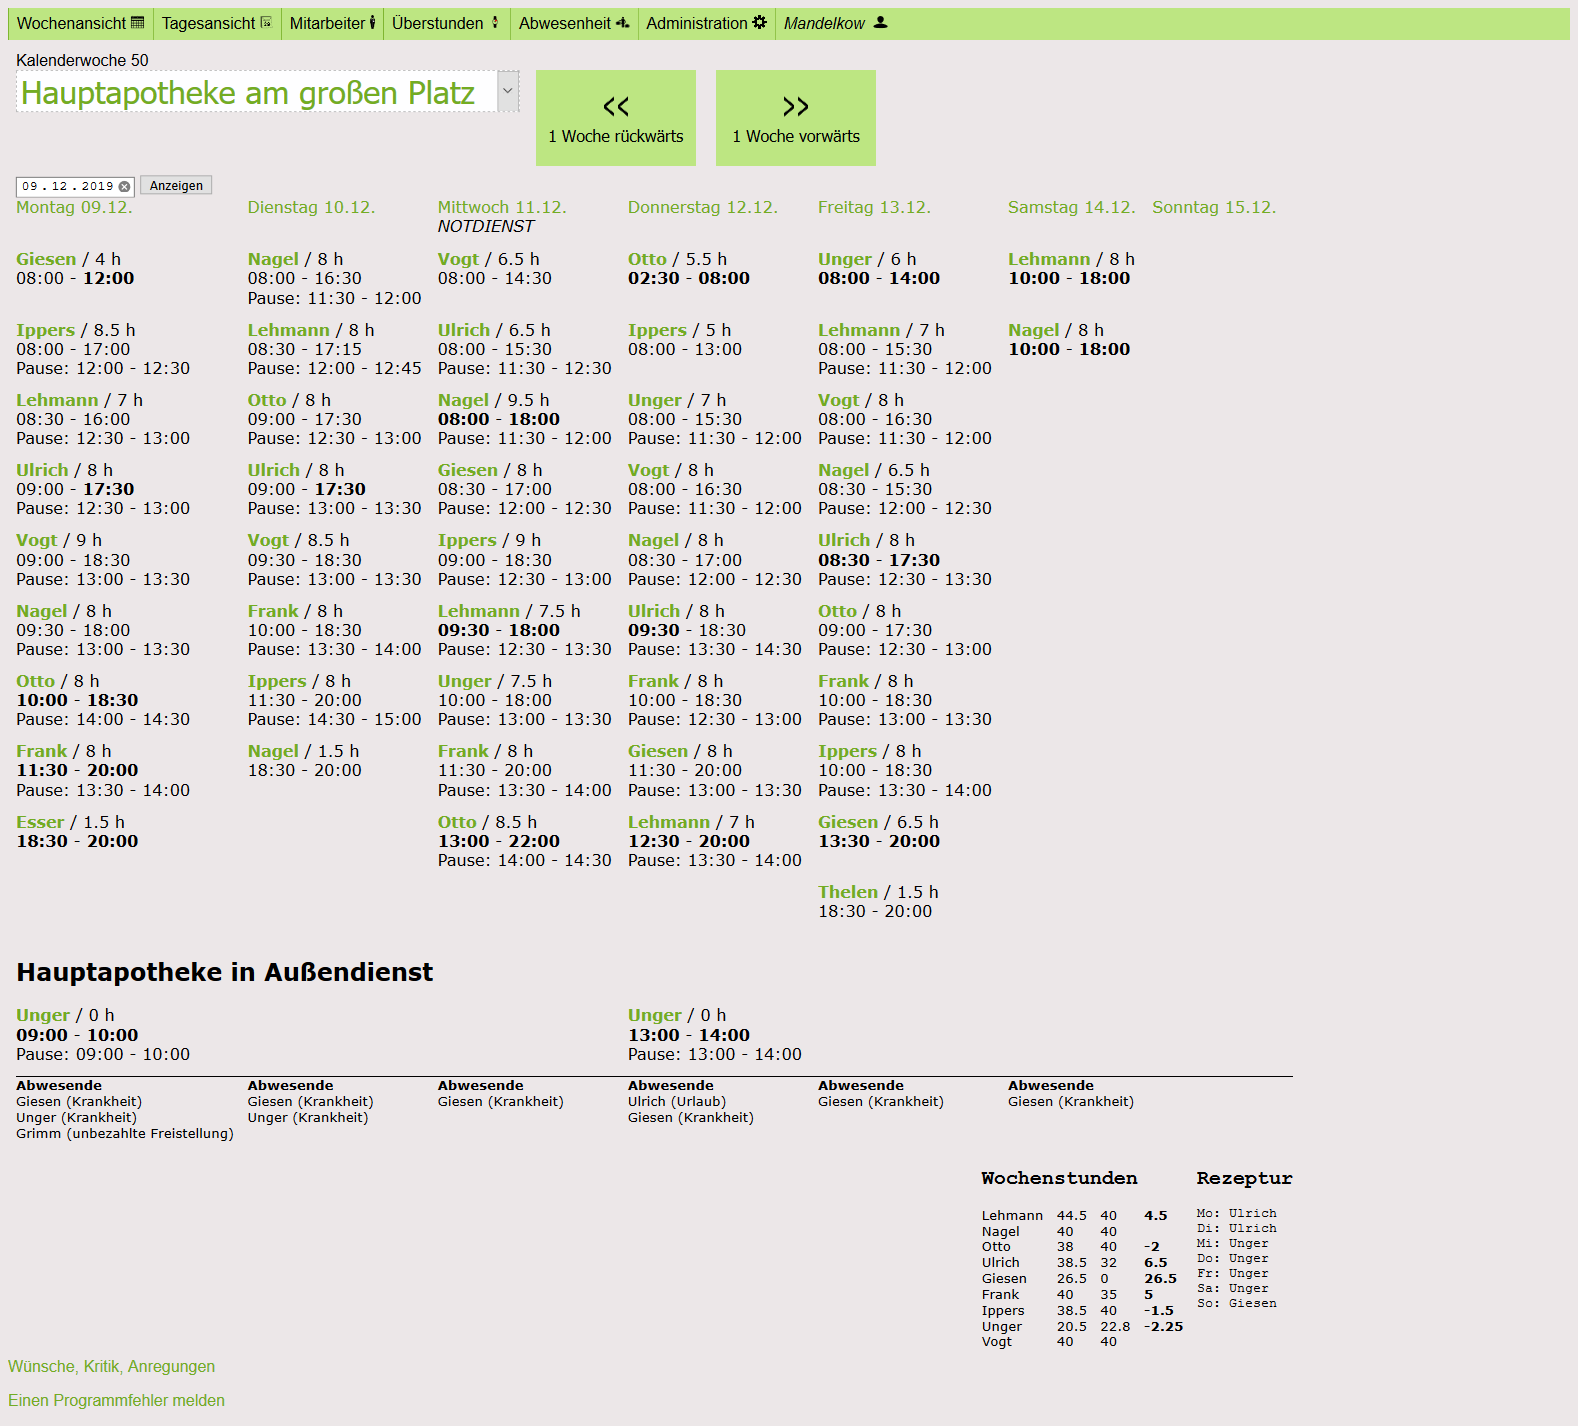
\includegraphics[width=0.8\linewidth]{{images/en_GB/roster-week-table.php}.png}
	\caption{Dienstplan Wochenansicht, Auszug ohne Aufgabenrotation und wöchentliche
Arbeitszeit}
	\label{img_roster_week_table_view}
\end{figure}

Die Dienstplan-Wochenansicht zeigt die Liste einer ausgewählten Woche und
Filiale (\autoref{img_roster_week_table_view}). Wenn Mitarbeiter der
Apotheke in einer anderen Filiale arbeiten, werden diese unten
angezeigt. Der Tabellenfuß enthält Informationen über abwesende Mitarbeiter
und deren Abwesenheitsgründe.

Das Datum kann durch direkte Eingabe ausgewählt werden. Es kann auch um eine
Woche vor oder zurück verschoben werden, indem man \keys{\ctrl + \shift +
\arrowkeyright} oder \keys {\ctrl + \shift + \arrowkeyleft} drückt.

\subsection{Dienstplan Tagesansicht}
\subsubsection{Schreibgeschützt}
In der Tageslistenansicht gibt es eine Tabelle, ein Balkendiagramm und ein
Histogramm, das den Dienstplan wiedergibt (\autoref{img_roster-day-read}).

\begin{figure}[h]
	\centering
	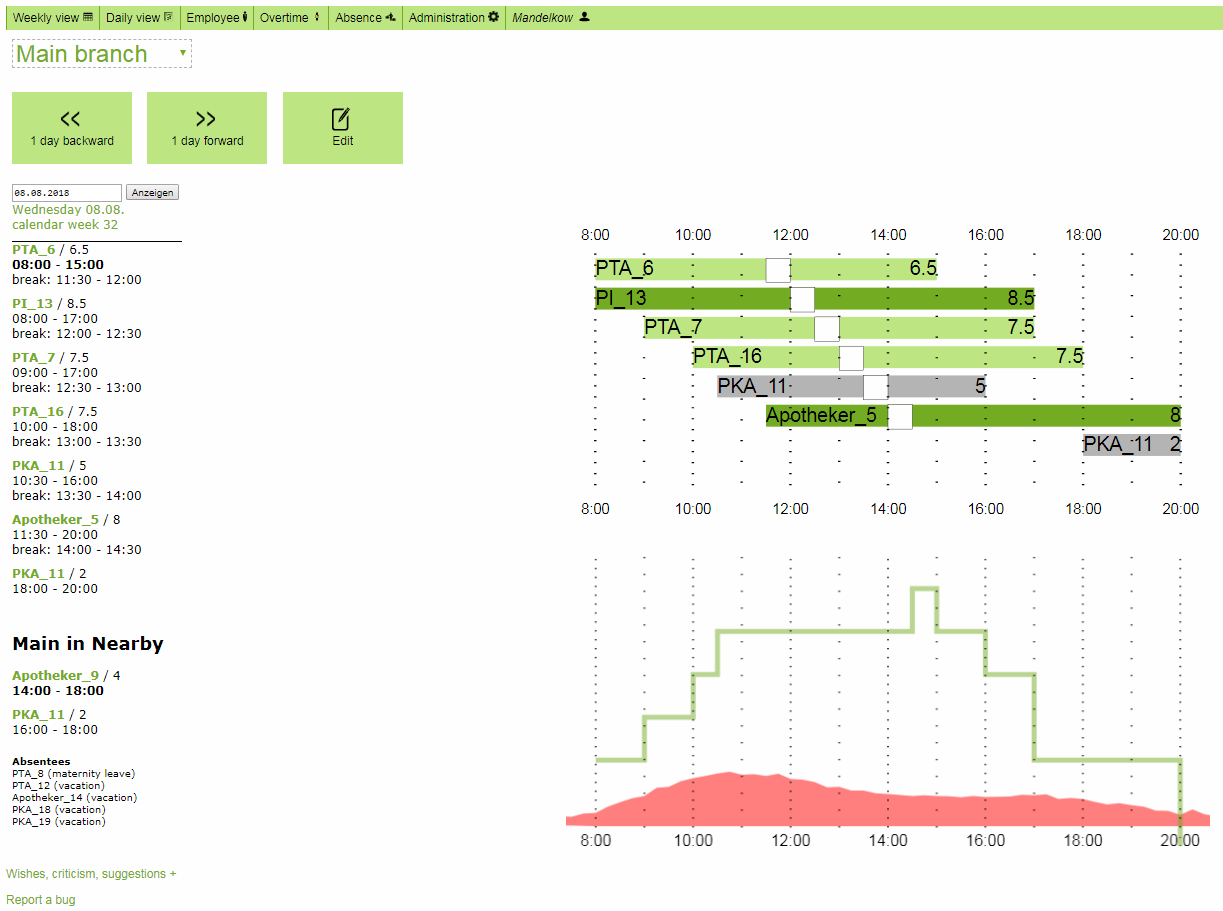
\includegraphics[width=0.8\linewidth]{{images/en_GB/roster-day-read.php}.png}
	\caption{Dienstplan Tagesansicht}
	\label{img_roster-day-read}
\end{figure}

Die Dienstplantabelle listet alle Mitarbeiter auf, die in dem ausgewählten
Zweig an dem ausgewählten Tag geplant sind. Jeder Eintrag enthält die ID und
den Nachnamen des Mitarbeiters, die Arbeitsstunden, den Beginn und das Ende
des Dienstes und die Zeit der Mittagspause, falls vorhanden.

Wenn ein Mitarbeiter, der in erster Linie in der ausgewählten Filiale
eingeplant ist, in einer anderen Filiale arbeitet, wird dieser Eintrag in
der Tabelle unten angezeigt. Ein Mitarbeiter kann mehr als einen Eintrag pro
Tag haben. Dadurch kann eine geteilte Arbeitszeit gespeichert werden. Wenn
Mitarbeiter abwesend sind, werden diese Abwesenheiten in der
Tabellenfußzeile angezeigt.


Das Dienstplan-Balken-Diagramm zeigt das Kommen und Gehen von
Mitarbeitern. Jeder Balken repräsentiert einen Eintrag. Er reicht vom Beginn
des Dienstes bis zu seinem Ende. Ein weißes Rechteck auf dem Balken zeigt
die Zeit der Mittagspause an. Die Farbe der Balken hängt vom Beruf des
Mitarbeiters ab. Apotheker und Pharmazieingenieure sind in dunkelgrün
gefärbt, während PTA in hellgrün gefärbt sind. Andere Mitarbeiter
(nichtpharmazeutisches Personal) sind grau hinterlegt.

Das Histogramm zeigt einen roten Bereich und eine grüne Linie. Der rote
Bereich zeigt den erwarteten Arbeitsaufwand (gemessen in Packungen pro 15
Minuten), während die grüne Linie die Anzahl der arbeitenden Mitarbeiter zu
einem bestimmten Zeitpunkt darstellt.


\subsubsection{Bearbeiten}
Die Bearbeitungsseite sieht der schreibgeschützten Ansicht sehr ähnlich
(\autoref{img_roster-day-edit}). 

\begin{figure}[h]
	\centering
	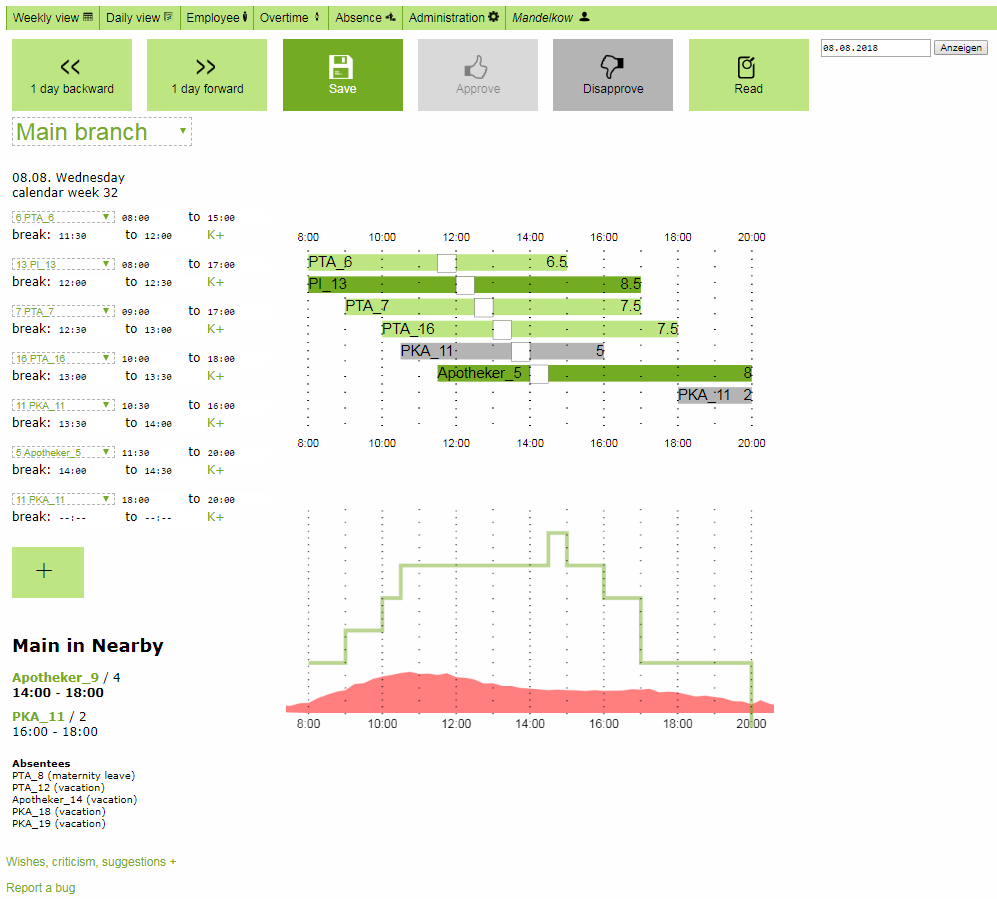
\includegraphics[width=0.8\linewidth]{{images/en_GB/roster-day-edit.php}.png}
	\caption{Dienstplanansicht mit Bearbeitungsrechten}
	\label{img_roster-day-edit}
\end{figure}

Der Dienstplan wird auf Fehler überprüft. Wenn Probleme auftreten, werden
Fehler, Warnungen oder Informationen im oberen rechten Bereich
angezeigt. Die Prüfung beinhaltet:
\begin{itemize}
    \item Überlappung von Schichten für denselben Mitarbeiter (Fehler)
    \item ausreichende Mitarbeiterzahl (Warnung, fest codiert mindestens zwei
Mitarbeiter)
    \item Anwesenheit von mindestens einem Apotheker zu jeder Zeit (Fehler).
    \item Anwesenheit von mindestens einer Person, die den Wareneingang durchführen
kann (Warnung).
    \item Einsatz abwesender Mitarbeiter (Fehler)
    \item Nichteinplanung von nicht abwesenden Mitarbeitern (Warnung)
\end{itemize}

Pro Eintrag kann nur eine Pause eingefügt werden. Wenn mehr Pausen
zugewiesen werden müssen, können mehrere Einträge für denselben Mitarbeiter
eingegeben werden.

\subsection{Dienstplan Mitarbeiteransicht}
Die Mitarbeiteransicht ähnelt der Wochenansicht, es wird jedoch nur ein
Mitarbeiter angezeigt (\autoref{img_roster-employee-table}).

\begin{figure}[h]
	\centering
	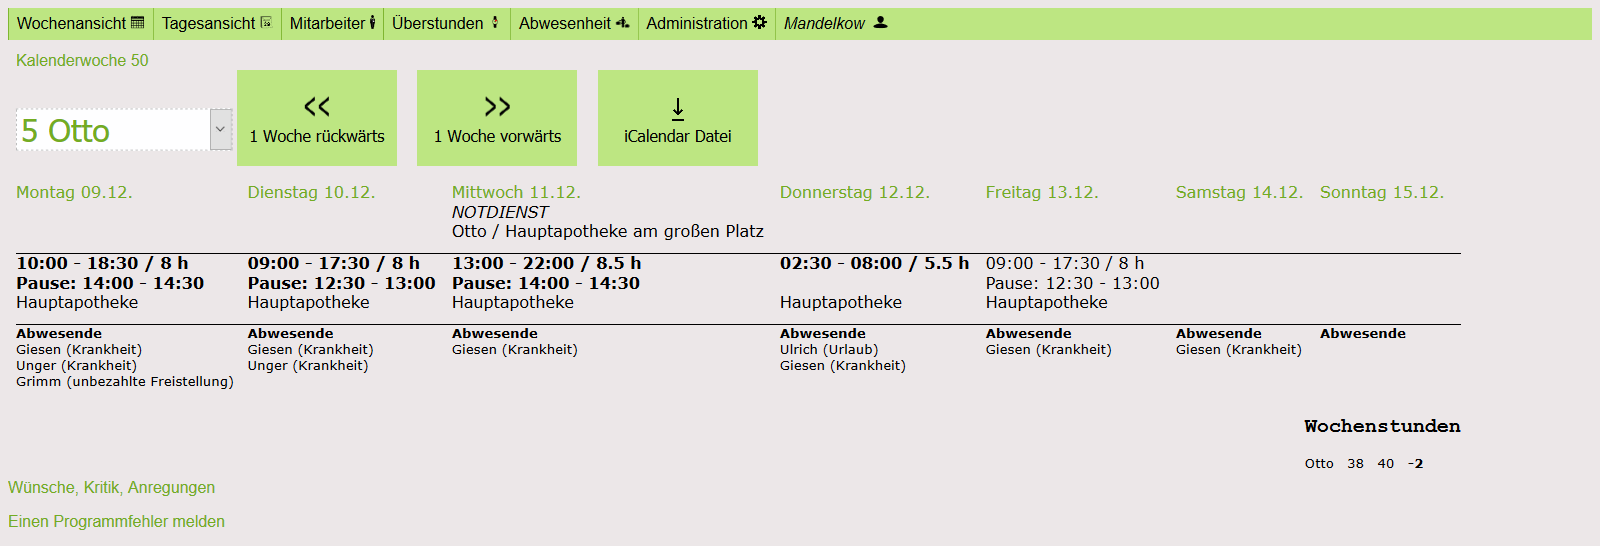
\includegraphics[width=0.8\linewidth]{{images/en_GB/roster-employee-table.php}.png}
	\caption{Mitarbeiteransicht}
	\label{img_roster-employee-table}
\end{figure}

Eine iCalendar-Datei kann heruntergeladen werden. Siehe
\autoref{section-calendar-api}~\nameref{section-calendar-api} für weitere
Informationen.

\subsection{Grundplan Tagesansicht}
Ein grundsätzlich wiederkehrender Dienstplan kann gespeichert werden. Im
einfachsten Fall handelt es sich dabei um eine Auflistung von Beginn und
Ende des Dienstes aller Mitarbeiter. Jeder Wochentag wird separat
aufgeführt, ebenso die Filialen.

Es ist möglich, abwechselnde Wochen zu erstellen. Beispielsweise kann eine
Mitarbeiterin in einer A-Woche und einer B-Woche arbeiten. In A-Wochen
beginnt sie am Montag regelmäßig um 08:00 Uhr, in B-Wochen um 10:00 Uhr.



\subsection{Überstunden}
\subsection{Abwesenheit}
Es gibt vier Ansichten zu den Abwesenheitsdaten.
\begin{itemize}
\item Mitarbeiteransicht schreibgeschützt
\item Mitarbeiteransicht Eingabe
\item Monatstabelle
\item Jahrestabelle
\end{itemize}
In der \emph{schreibgeschützten Mitarbeitersicht} gibt es ein
Select-Element, um den anzuzeigenden Mitarbeiter auszuwählen. Es gibt eine
Schaltfläche, um zur Bearbeitungsansicht zu wechseln. Und es gibt eine
Tabelle mit den Abwesenheitsdaten. Die Spalten sind Beginn und Ende der
Abwesenheit, Abwesenheitsgrund und Anzahl der Tage. Es gibt eine eindeutige
Liste möglicher Gründe (Urlaub, Resturlaub, Krankheit, Krankheit des Kindes,
unbezahlte Freistellung, bezahlte Freistellung, Elternzeit und
Mutterschutz). Die Anzahl der Abwesenheitstage wird für eine 5-Tage-Woche
berechnet. Abwesenheiten an Samstagen und Sonntagen werden registriert, aber
nicht gezählt. Das Gleiche gilt für Feiertage.



\section{Kalender API}\label{section-calendar-api}
Es ist möglich, die Dienstplandaten in Form von iCalendar-Dateien von PDR zu
lesen. Diese Dateien können mit allen wichtigen Kalenderanwendungen auf
Desktops und Smartphones verwendet werden. Diese API ist keinesfalls eine
vollständige Implementierung des Webdav-Standards. Es ist nicht einmal eine
Implementierung des CalDAV-Protokolls. Rufen Sie in Ihrem Browser einfach
auf die folgende URL auf: \url{https://YOURHOSTNAME/YOUR/FOLDER/webdav.php}


Die Optionen sind:
\begin{description}
	\item \lstinline|employee_id| Die Mitarbeiter-ID des Benutzers, von dem der
Dienstplan ausgegeben werden soll. Jeder Benutzer kann die Liste aller
Mitarbeiter abrufen. (Standard = der angemeldete Benutzer)
	\item \lstinline|date_string| Ein Datum im Format JJJJ-MM-TT (Standard = heute)
	\item \lstinline|days_into_the_future| Die Anzahl der Tage, die in der
Kalenderdatei enthalten sein sollen. (Standard = 30)
	\item \lstinline|create_valarm| Erstellen Sie einen Alarm
(\lstinline|ACTION:DISPLAY|) auf Ihrem Gerät. (Standard = 0)
	\begin{itemize}
        \item 0 = kein Alarm
        \item 1 = Alarm 30 Minuten vor Dienstantritt
        \item 2 = Alarm am Ende des Dienstes
        \item 4 = Alarm, wenn die Mittagspause beginnt
        \item 8 = Alarm, wenn die Mittagspause endet
        \item 11 = 1+2+8 = Alarm für Beginn und Ende des Dienstes sowie für das Ende des
Mittagessens, jedoch nicht für den Beginn des Mittagessens
    \end{itemize}	
\end{description}	

Um den Dienstplan der Woche ab 17.12.2018 für den Angestellten Nummer 5 zu
erhalten, verwenden Sie die folgende URL:
\url{https://YOURHOSTNAME/YOUR/FOLDER/webdav.php?employee_id=5&date_string=2018-12-17&days_into_the_future=6}

\subsection{ICalendar-Dateien automatisch mit  "iCal Import/Export CalDAV Pro"
importieren}
Der automatische Import von iCalendar-Dateien in Android-Smartphones wurde
mit "iCal Import/Export CalDAV Pro" (3,59 EUR) getestet. Es gibt
wahrscheinlich andere Apps, die das Selbe tun können.

\begin{figure}[hbtp]
    \centering
    \begin{minipage}{0.45\textwidth}
        \centering
	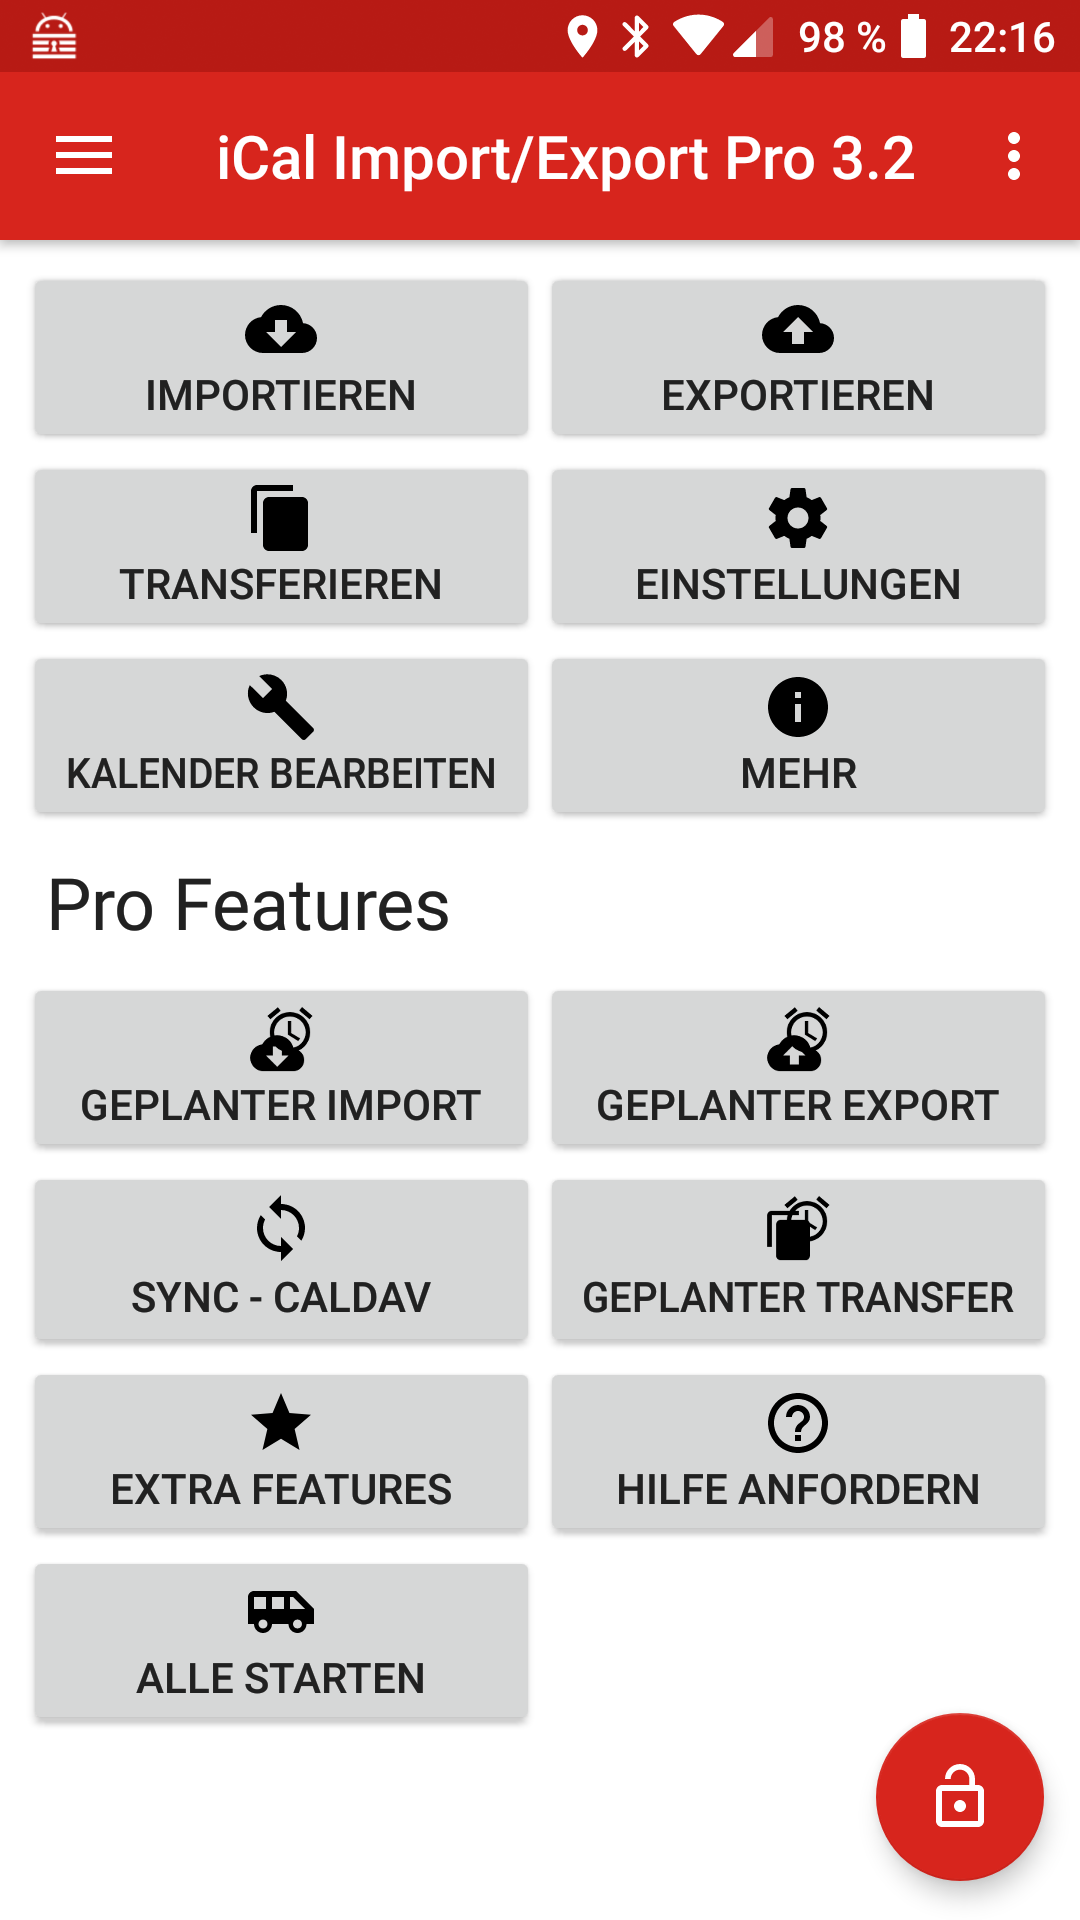
\includegraphics[width=0.9\textwidth, height=0.3\textheight, keepaspectratio=true]{{images/de_DE/iCalendar_import_0.png}}
	\caption{iCal Hauptmenü}
    \end{minipage}\hfill
    \begin{minipage}{0.45\textwidth}
        \centering
	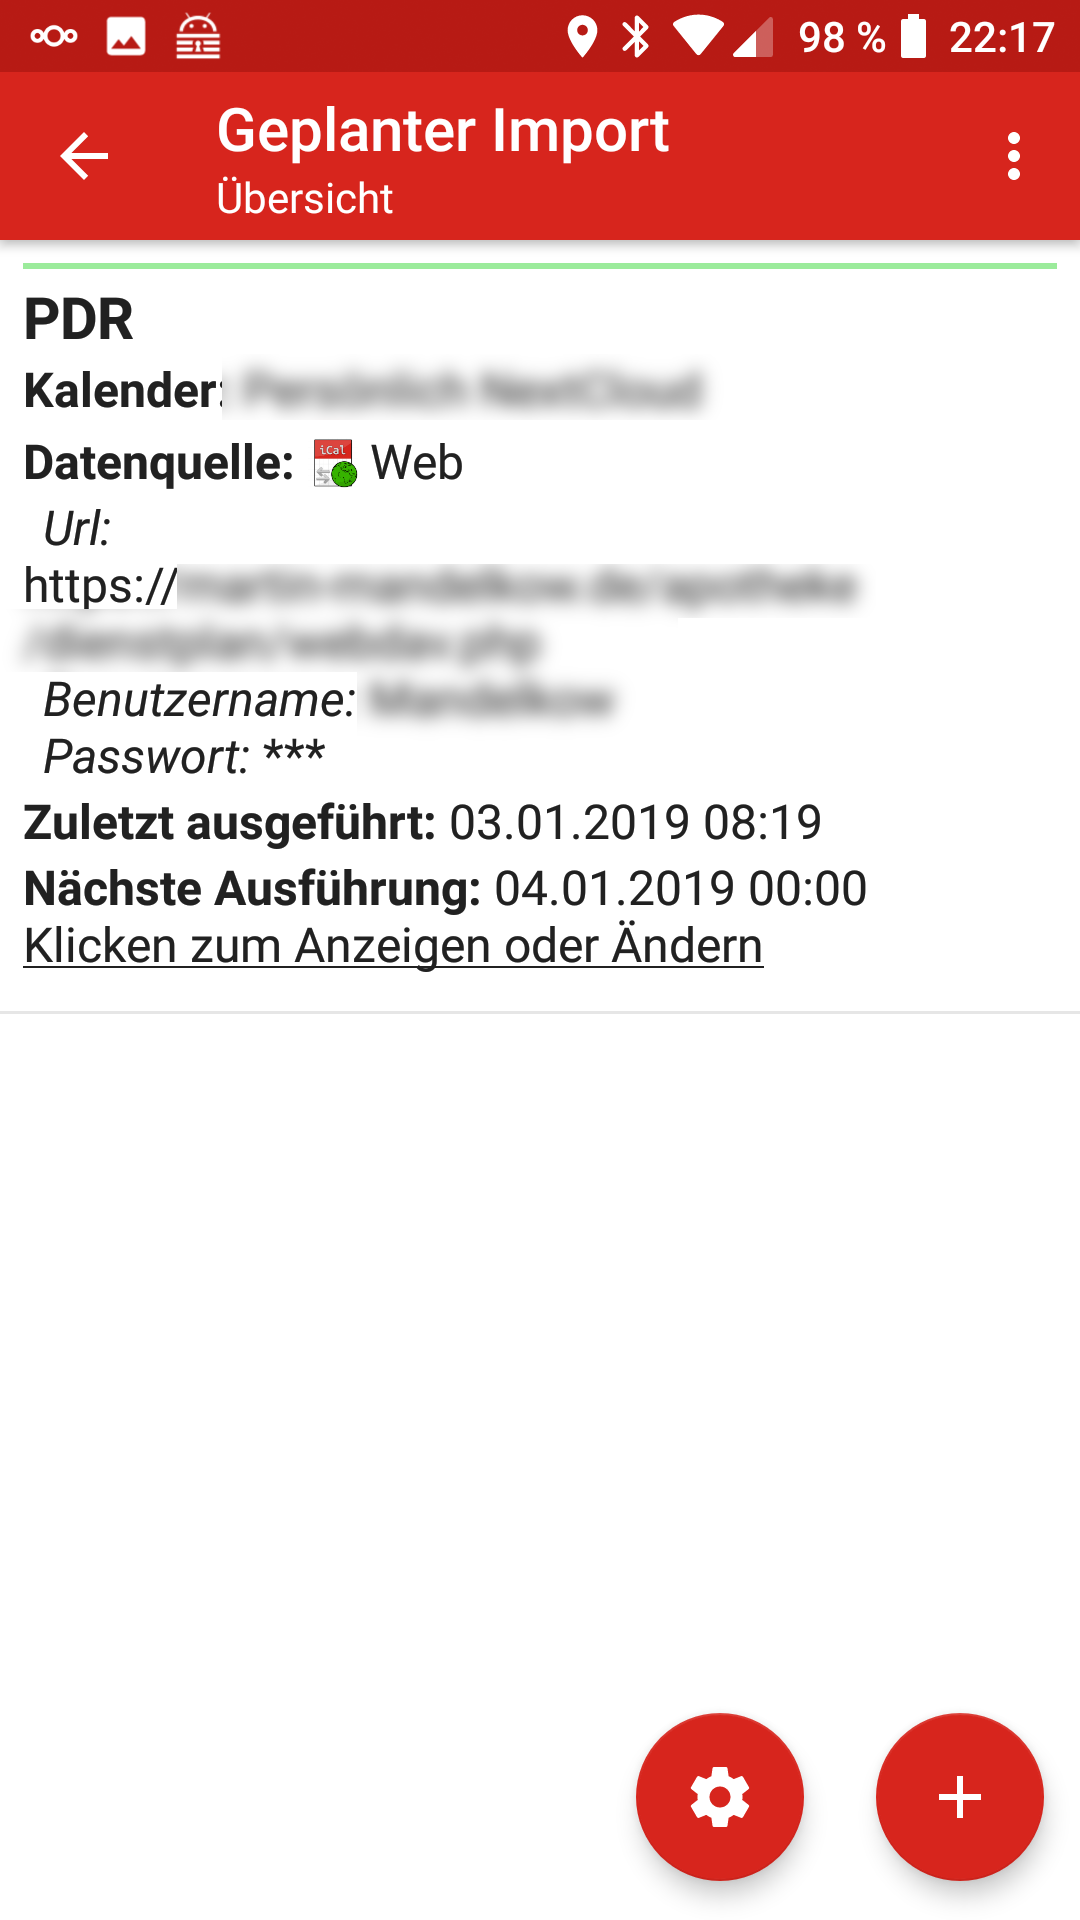
\includegraphics[width=0.9\textwidth, height=0.3\textheight, keepaspectratio=true]{{images/de_DE/iCalendar_import_1.png}}
	\caption{iCal geplante Importe}
    \end{minipage}
    \vfill
    \centering
    \begin{minipage}{0.45\textwidth}
        \centering
	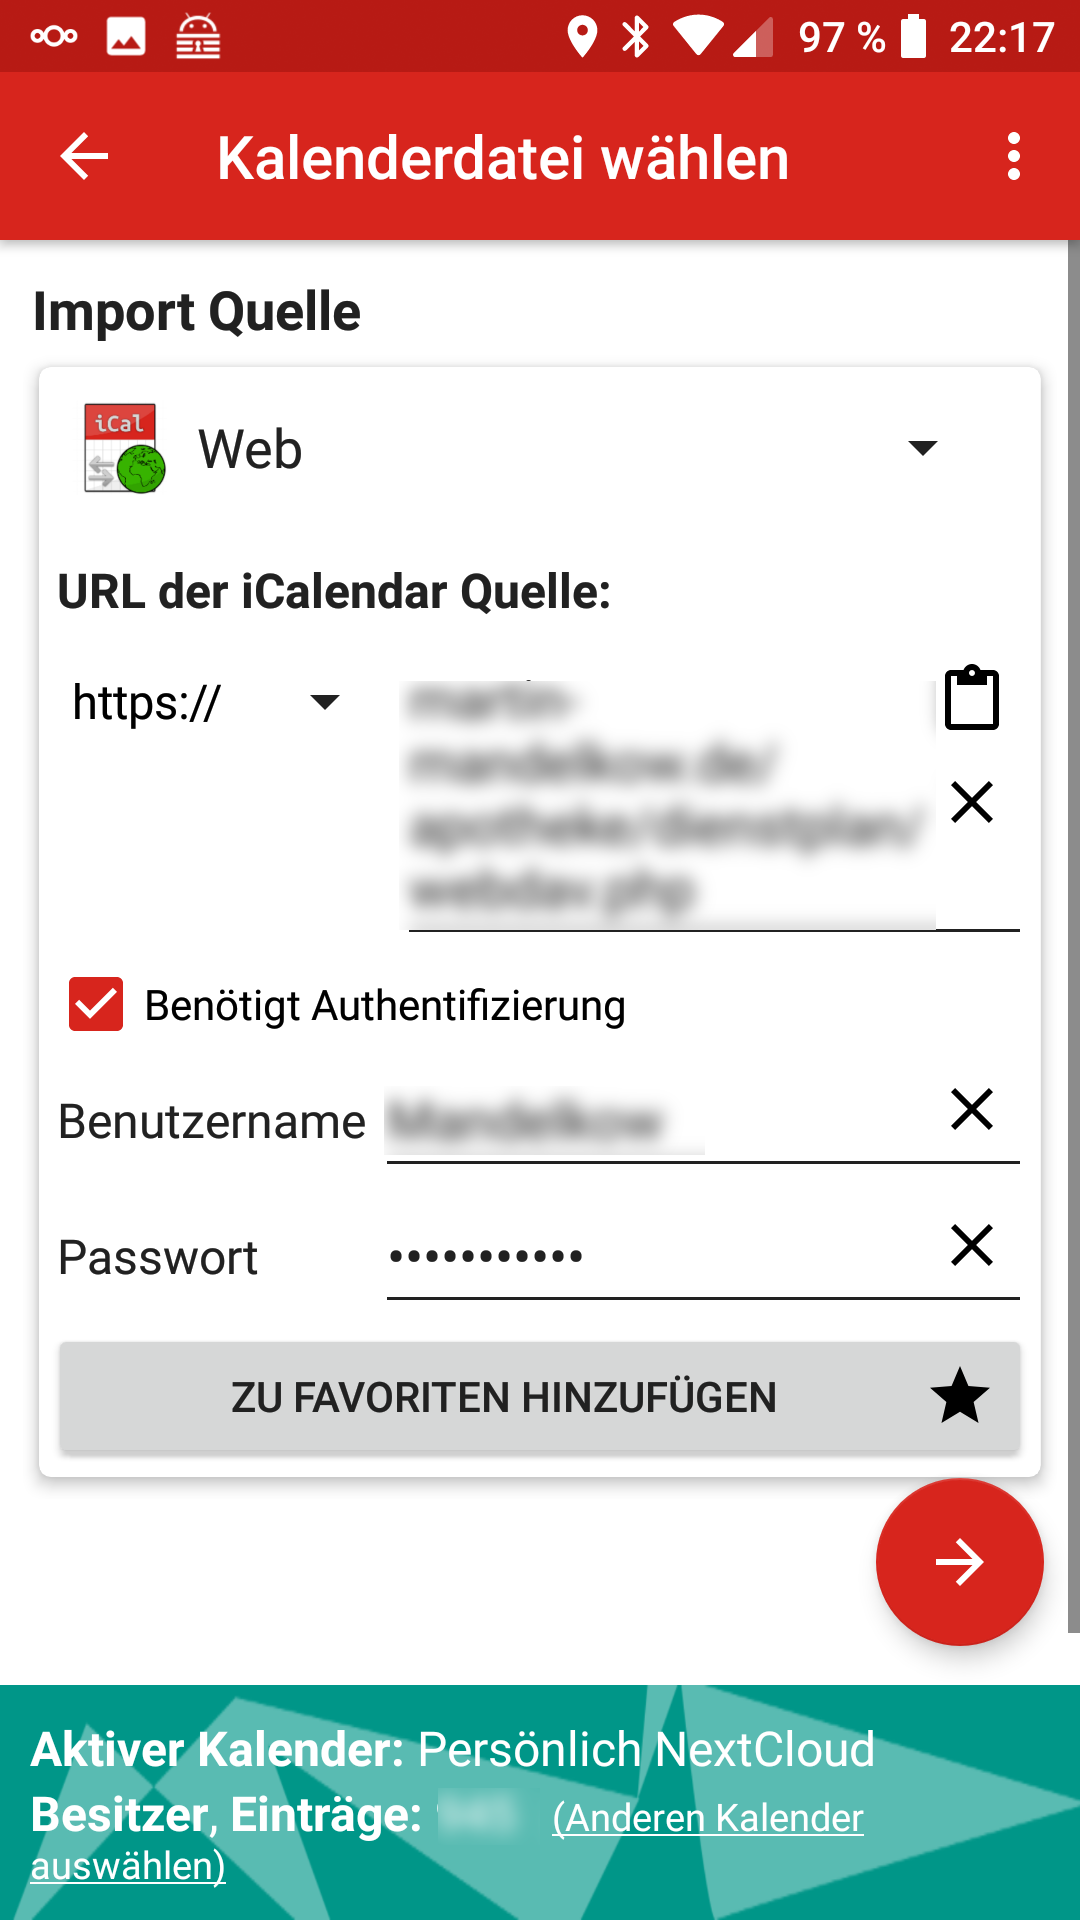
\includegraphics[width=0.9\textwidth, height=0.3\textheight, keepaspectratio=true]{{images/de_DE/iCalendar_import_2.png}}
	\caption{iCal eine neue Importquelle hinzufügen}
    \end{minipage}\hfill
    \begin{minipage}{0.45\textwidth}
        \centering
	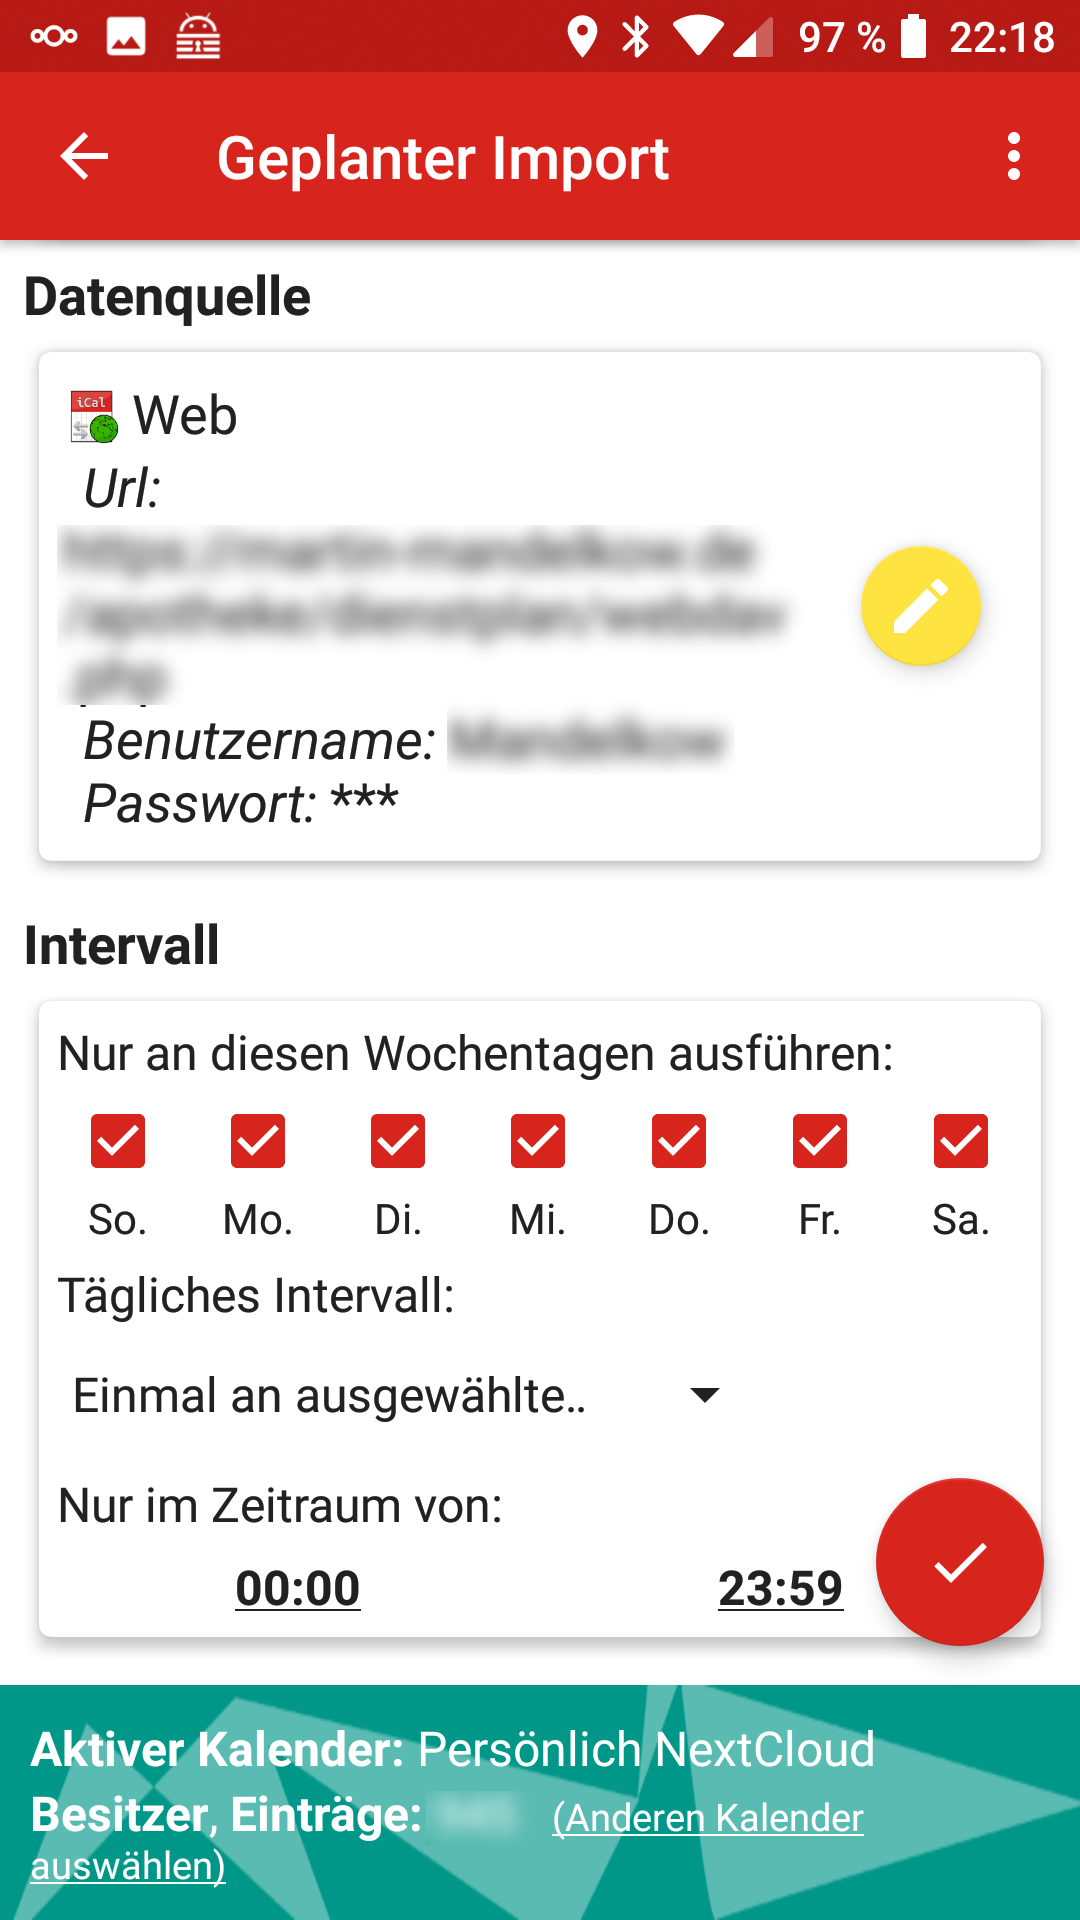
\includegraphics[width=0.9\textwidth, height=0.3\textheight, keepaspectratio=true]{{images/de_DE/iCalendar_import_3.png}}
	\caption{iCal Importintervalle einstellen}
    \end{minipage}
    \begin{minipage}{0.45\textwidth}
        \centering
	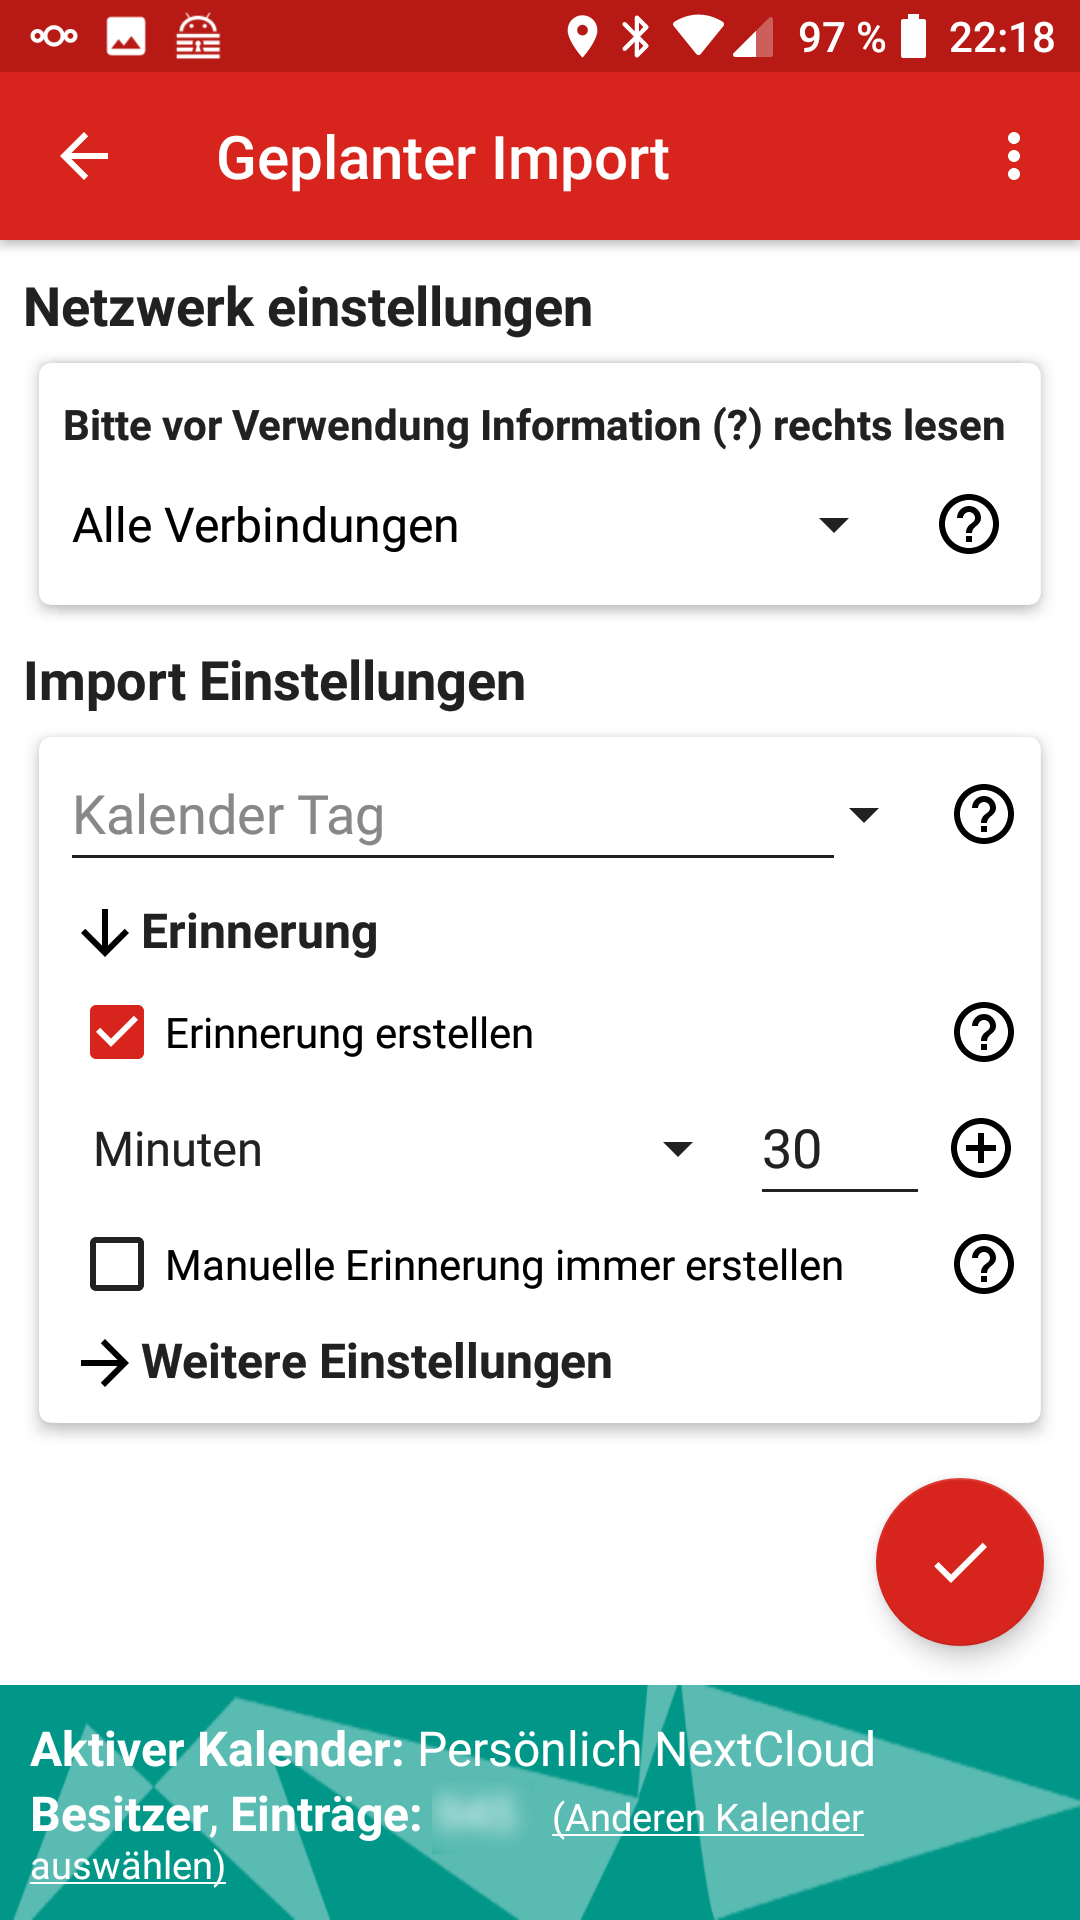
\includegraphics[width=0.9\textwidth, height=0.3\textheight, keepaspectratio=true]{{images/de_DE/iCalendar_import_4.png}}
	\caption{iCal Netzwerkeinstellungen und Importeinstellungen}
    \end{minipage}
\end{figure}
